% REV01 Tue 04 May 2021 13:34:33 WIB
% START Sat 27 Mar 2021 06:21:38 WIB

\chapter{CUT ADRIFT}

The Six Jolly Fellowship Porters, already mentioned as a tavern of
a dropsical appearance, had long settled down into a state of hale
infirmity. In its whole constitution it had not a straight floor, and
hardly a straight line; but it had outlasted, and clearly would yet
outlast, many a better-trimmed building, many a sprucer public-house.
Externally, it was a narrow lopsided wooden jumble of corpulent windows
heaped one upon another as you might heap as many toppling oranges,
with a crazy wooden verandah impending over the water; indeed the whole
house, inclusive of the complaining flag-staff on the roof, impended
over the water, but seemed to have got into the condition of a
faint-hearted diver who has paused so long on the brink that he will
never go in at all.

This description applies to the river-frontage of the Six Jolly
Fellowship Porters. The back of the establishment, though the chief
entrance was there, so contracted that it merely represented in its
connexion with the front, the handle of a flat iron set upright on its
broadest end. This handle stood at the bottom of a wilderness of court
and alley: which wilderness pressed so hard and close upon the Six Jolly
Fellowship Porters as to leave the hostelry not an inch of ground beyond
its door. For this reason, in combination with the fact that the house
was all but afloat at high water, when the Porters had a family wash the
linen subjected to that operation might usually be seen drying on lines
stretched across the reception-rooms and bed-chambers.

The wood forming the chimney-pieces, beams, partitions, floors and
doors, of the Six Jolly Fellowship Porters, seemed in its old age
fraught with confused memories of its youth. In many places it had
become gnarled and riven, according to the manner of old trees; knots
started out of it; and here and there it seemed to twist itself into
some likeness of boughs. In this state of second childhood, it had an
air of being in its own way garrulous about its early life. Not without
reason was it often asserted by the regular frequenters of the Porters,
that when the light shone full upon the grain of certain panels, and
particularly upon an old corner cupboard of walnut-wood in the bar, you
might trace little forests there, and tiny trees like the parent tree,
in full umbrageous leaf.

The bar of the Six Jolly Fellowship Porters was a bar to soften the
human breast. The available space in it was not much larger than a
hackney-coach; but no one could have wished the bar bigger, that space
was so girt in by corpulent little casks, and by cordial-bottles
radiant with fictitious grapes in bunches, and by lemons in nets, and
by biscuits in baskets, and by the polite beer-pulls that made low
bows when customers were served with beer, and by the cheese in a snug
corner, and by the landlady’s own small table in a snugger corner near
the fire, with the cloth everlastingly laid. This haven was divided from
the rough world by a glass partition and a half-door, with a leaden
sill upon it for the convenience of resting your liquor; but, over this
half-door the bar’s snugness so gushed forth that, albeit customers
drank there standing, in a dark and draughty passage where they were
shouldered by other customers passing in and out, they always appeared
to drink under an enchanting delusion that they were in the bar itself.

For the rest, both the tap and parlour of the Six Jolly Fellowship
Porters gave upon the river, and had red curtains matching the noses of
the regular customers, and were provided with comfortable fireside tin
utensils, like models of sugar-loaf hats, made in that shape that they
might, with their pointed ends, seek out for themselves glowing nooks
in the depths of the red coals, when they mulled your ale, or heated for
you those delectable drinks, Purl, Flip, and Dog’s Nose. The first of
these humming compounds was a speciality of the Porters, which, through
an inscription on its door-posts, gently appealed to your feelings as,
‘The Early Purl House’. For, it would seem that Purl must always be
taken early; though whether for any more distinctly stomachic reason
than that, as the early bird catches the worm, so the early purl catches
the customer, cannot here be resolved. It only remains to add that in
the handle of the flat iron, and opposite the bar, was a very little
room like a three-cornered hat, into which no direct ray of sun, moon,
or star, ever penetrated, but which was superstitiously regarded as a
sanctuary replete with comfort and retirement by gaslight, and on the
door of which was therefore painted its alluring name: Cosy.

Miss Potterson, sole proprietor and manager of the Fellowship Porters,
reigned supreme on her throne, the Bar, and a man must have drunk
himself mad drunk indeed if he thought he could contest a point with
her. Being known on her own authority as Miss Abbey Potterson, some
water-side heads, which (like the water) were none of the clearest,
harboured muddled notions that, because of her dignity and firmness, she
was named after, or in some sort related to, the Abbey at Westminster.
But, Abbey was only short for Abigail, by which name Miss Potterson had
been christened at Limehouse Church, some sixty and odd years before.

‘Now, you mind, you Riderhood,’ said Miss Abbey Potterson, with emphatic
forefinger over the half-door, ‘the Fellowship don’t want you at all,
and would rather by far have your room than your company; but if you
were as welcome here as you are not, you shouldn’t even then have
another drop of drink here this night, after this present pint of beer.
So make the most of it.’

‘But you know, Miss Potterson,’ this was suggested very meekly though,
‘if I behave myself, you can’t help serving me, miss.’

‘CAN’T I!’ said Abbey, with infinite expression.

‘No, Miss Potterson; because, you see, the law--’

‘I am the law here, my man,’ returned Miss Abbey, ‘and I’ll soon
convince you of that, if you doubt it at all.’

‘I never said I did doubt it at all, Miss Abbey.’

‘So much the better for you.’

Abbey the supreme threw the customer’s halfpence into the till, and,
seating herself in her fireside-chair, resumed the newspaper she had
been reading. She was a tall, upright, well-favoured woman, though
severe of countenance, and had more of the air of a schoolmistress than
mistress of the Six Jolly Fellowship Porters. The man on the other side
of the half-door, was a waterside-man with a squinting leer, and he eyed
her as if he were one of her pupils in disgrace.

‘You’re cruel hard upon me, Miss Potterson.’

Miss Potterson read her newspaper with contracted brows, and took no
notice until he whispered:

‘Miss Potterson! Ma’am! Might I have half a word with you?’

Deigning then to turn her eyes sideways towards the suppliant, Miss
Potterson beheld him knuckling his low forehead, and ducking at her with
his head, as if he were asking leave to fling himself head foremost over
the half-door and alight on his feet in the bar.

‘Well?’ said Miss Potterson, with a manner as short as she herself was
long, ‘say your half word. Bring it out.’

‘Miss Potterson! Ma’am! Would you ‘sxcuse me taking the liberty of
asking, is it my character that you take objections to?’

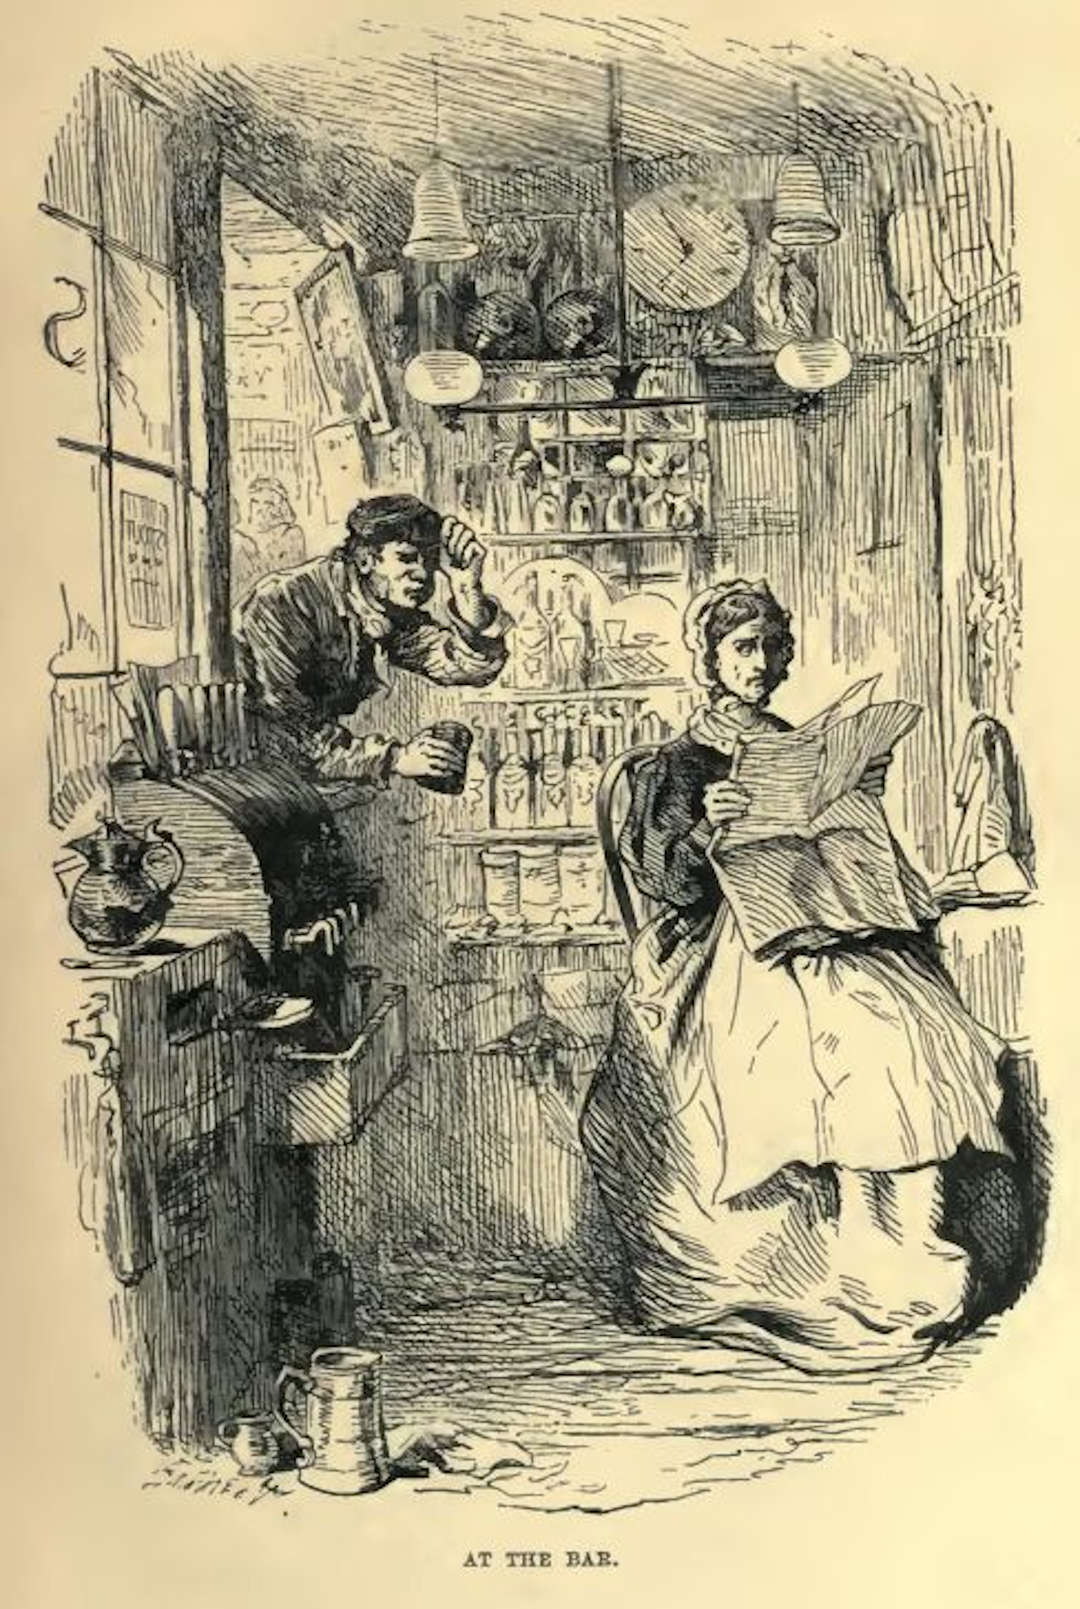
\includegraphics[scale=2.3]{01-06-01}

‘Certainly,’ said Miss Potterson.

‘Is it that you’re afraid of--’

‘I am not afraid OF YOU,’ interposed Miss Potterson, ‘if you mean that.’

‘But I humbly don’t mean that, Miss Abbey.’

‘Then what do you mean?’

‘You really are so cruel hard upon me! What I was going to make
inquiries was no more than, might you have any apprehensions--leastways
beliefs or suppositions--that the company’s property mightn’t be
altogether to be considered safe, if I used the house too regular?’

‘What do you want to know for?’

‘Well, Miss Abbey, respectfully meaning no offence to you, it would
be some satisfaction to a man’s mind, to understand why the Fellowship
Porters is not to be free to such as me, and is to be free to such as
Gaffer.’

The face of the hostess darkened with some shadow of perplexity, as she
replied: ‘Gaffer has never been where you have been.’

‘Signifying in Quod, Miss? Perhaps not. But he may have merited it. He
may be suspected of far worse than ever I was.’

‘Who suspects him?’

‘Many, perhaps. One, beyond all doubts. I do.’

‘YOU are not much,’ said Miss Abbey Potterson, knitting her brows again
with disdain.

‘But I was his pardner. Mind you, Miss Abbey, I was his pardner. As
such I know more of the ins and outs of him than any person living does.
Notice this! I am the man that was his pardner, and I am the man that
suspects him.’

‘Then,’ suggested Miss Abbey, though with a deeper shade of perplexity
than before, ‘you criminate yourself.’

‘No I don’t, Miss Abbey. For how does it stand? It stands this way. When
I was his pardner, I couldn’t never give him satisfaction. Why couldn’t
I never give him satisfaction? Because my luck was bad; because I
couldn’t find many enough of ‘em. How was his luck? Always good. Notice
this! Always good! Ah! There’s a many games, Miss Abbey, in which
there’s chance, but there’s a many others in which there’s skill too,
mixed along with it.’

‘That Gaffer has a skill in finding what he finds, who doubts, man?’
asked Miss Abbey.

‘A skill in purwiding what he finds, perhaps,’ said Riderhood, shaking
his evil head.

Miss Abbey knitted her brow at him, as he darkly leered at her. ‘If
you’re out upon the river pretty nigh every tide, and if you want to
find a man or woman in the river, you’ll greatly help your luck, Miss
Abbey, by knocking a man or woman on the head aforehand and pitching ‘em
in.’

‘Gracious Lud!’ was the involuntary exclamation of Miss Potterson.

‘Mind you!’ returned the other, stretching forward over the half door
to throw his words into the bar; for his voice was as if the head of his
boat’s mop were down his throat; ‘I say so, Miss Abbey! And mind you!
I’ll follow him up, Miss Abbey! And mind you! I’ll bring him to hook at
last, if it’s twenty year hence, I will! Who’s he, to be favoured along
of his daughter? Ain’t I got a daughter of my own!’

With that flourish, and seeming to have talked himself rather more drunk
and much more ferocious than he had begun by being, Mr Riderhood took up
his pint pot and swaggered off to the taproom.

Gaffer was not there, but a pretty strong muster of Miss Abbey’s pupils
were, who exhibited, when occasion required, the greatest docility. On
the clock’s striking ten, and Miss Abbey’s appearing at the door, and
addressing a certain person in a faded scarlet jacket, with ‘George
Jones, your time’s up! I told your wife you should be punctual,’
Jones submissively rose, gave the company good-night, and retired. At
half-past ten, on Miss Abbey’s looking in again, and saying, ‘William
Williams, Bob Glamour, and Jonathan, you are all due,’ Williams, Bob,
and Jonathan with similar meekness took their leave and evaporated.
Greater wonder than these, when a bottle-nosed person in a glazed hat
had after some considerable hesitation ordered another glass of gin and
water of the attendant potboy, and when Miss Abbey, instead of sending
it, appeared in person, saying, ‘Captain Joey, you have had as much as
will do you good,’ not only did the captain feebly rub his knees and
contemplate the fire without offering a word of protest, but the rest
of the company murmured, ‘Ay, ay, Captain! Miss Abbey’s right; you
be guided by Miss Abbey, Captain.’ Nor, was Miss Abbey’s vigilance in
anywise abated by this submission, but rather sharpened; for, looking
round on the deferential faces of her school, and descrying two other
young persons in need of admonition, she thus bestowed it: ‘Tom Tootle,
it’s time for a young fellow who’s going to be married next month, to
be at home and asleep. And you needn’t nudge him, Mr Jack Mullins, for
I know your work begins early tomorrow, and I say the same to you.
So come! Good-night, like good lads!’ Upon which, the blushing Tootle
looked to Mullins, and the blushing Mullins looked to Tootle, on the
question who should rise first, and finally both rose together and went
out on the broad grin, followed by Miss Abbey; in whose presence the
company did not take the liberty of grinning likewise.

In such an establishment, the white-aproned pot-boy with his
shirt-sleeves arranged in a tight roll on each bare shoulder, was a mere
hint of the possibility of physical force, thrown out as a matter of
state and form. Exactly at the closing hour, all the guests who were
left, filed out in the best order: Miss Abbey standing at the half door
of the bar, to hold a ceremony of review and dismissal. All wished
Miss Abbey good-night and Miss Abbey wished good-night to all, except
Riderhood. The sapient pot-boy, looking on officially, then had the
conviction borne in upon his soul, that the man was evermore outcast and
excommunicate from the Six Jolly Fellowship Porters.

‘You Bob Gliddery,’ said Miss Abbey to this pot-boy, ‘run round to
Hexam’s and tell his daughter Lizzie that I want to speak to her.’

With exemplary swiftness Bob Gliddery departed, and returned. Lizzie,
following him, arrived as one of the two female domestics of the
Fellowship Porters arranged on the snug little table by the bar fire,
Miss Potterson’s supper of hot sausages and mashed potatoes.

‘Come in and sit ye down, girl,’ said Miss Abbey. ‘Can you eat a bit?’

‘No thank you, Miss. I have had my supper.’

‘I have had mine too, I think,’ said Miss Abbey, pushing away the
untasted dish, ‘and more than enough of it. I am put out, Lizzie.’

‘I am very sorry for it, Miss.’

‘Then why, in the name of Goodness,’ quoth Miss Abbey, sharply, ‘do you
do it?’

‘I do it, Miss!’

‘There, there. Don’t look astonished. I ought to have begun with a word
of explanation, but it’s my way to make short cuts at things. I always
was a pepperer. You Bob Gliddery there, put the chain upon the door and
get ye down to your supper.’

With an alacrity that seemed no less referable to the pepperer fact
than to the supper fact, Bob obeyed, and his boots were heard descending
towards the bed of the river.

‘Lizzie Hexam, Lizzie Hexam,’ then began Miss Potterson, ‘how often have
I held out to you the opportunity of getting clear of your father, and
doing well?’

‘Very often, Miss.’

‘Very often? Yes! And I might as well have spoken to the iron funnel of
the strongest sea-going steamer that passes the Fellowship Porters.’

‘No, Miss,’ Lizzie pleaded; ‘because that would not be thankful, and I
am.’

‘I vow and declare I am half ashamed of myself for taking such an
interest in you,’ said Miss Abbey, pettishly, ‘for I don’t believe I
should do it if you were not good-looking. Why ain’t you ugly?’

Lizzie merely answered this difficult question with an apologetic
glance.

‘However, you ain’t,’ resumed Miss Potterson, ‘so it’s no use going into
that. I must take you as I find you. Which indeed is what I’ve done. And
you mean to say you are still obstinate?’

‘Not obstinate, Miss, I hope.’

‘Firm (I suppose you call it) then?’

‘Yes, Miss. Fixed like.’

‘Never was an obstinate person yet, who would own to the word!’ remarked
Miss Potterson, rubbing her vexed nose; ‘I’m sure I would, if I was
obstinate; but I am a pepperer, which is different. Lizzie Hexam, Lizzie
Hexam, think again. Do you know the worst of your father?’

‘Do I know the worst of father!’ she repeated, opening her eyes.

‘Do you know the suspicions to which your father makes himself liable?
Do you know the suspicions that are actually about, against him?’

The consciousness of what he habitually did, oppressed the girl heavily,
and she slowly cast down her eyes.

‘Say, Lizzie. Do you know?’ urged Miss Abbey.

‘Please to tell me what the suspicions are, Miss,’ she asked after a
silence, with her eyes upon the ground.

‘It’s not an easy thing to tell a daughter, but it must be told. It is
thought by some, then, that your father helps to their death a few of
those that he finds dead.’

The relief of hearing what she felt sure was a false suspicion, in place
of the expected real and true one, so lightened Lizzie’s breast for the
moment, that Miss Abbey was amazed at her demeanour. She raised her eyes
quickly, shook her head, and, in a kind of triumph, almost laughed.

‘They little know father who talk like that!’

[‘She takes it,’ thought Miss Abbey, ‘very quietly. She takes it with
extraordinary quietness!’)

‘And perhaps,’ said Lizzie, as a recollection flashed upon her, ‘it is
some one who has a grudge against father; some one who has threatened
father! Is it Riderhood, Miss?’

‘Well; yes it is.’

‘Yes! He was father’s partner, and father broke with him, and now he
revenges himself. Father broke with him when I was by, and he was very
angry at it. And besides, Miss Abbey!--Will you never, without strong
reason, let pass your lips what I am going to say?’

She bent forward to say it in a whisper.

‘I promise,’ said Miss Abbey.

‘It was on the night when the Harmon murder was found out, through
father, just above bridge. And just below bridge, as we were sculling
home, Riderhood crept out of the dark in his boat. And many and many
times afterwards, when such great pains were taken to come to the bottom
of the crime, and it never could be come near, I thought in my own
thoughts, could Riderhood himself have done the murder, and did he
purposely let father find the body? It seemed a’most wicked and cruel
to so much as think such a thing; but now that he tries to throw it upon
father, I go back to it as if it was a truth. Can it be a truth? That
was put into my mind by the dead?’

She asked this question, rather of the fire than of the hostess of the
Fellowship Porters, and looked round the little bar with troubled eyes.

But, Miss Potterson, as a ready schoolmistress accustomed to bring her
pupils to book, set the matter in a light that was essentially of this
world.

‘You poor deluded girl,’ she said, ‘don’t you see that you can’t open
your mind to particular suspicions of one of the two, without opening
your mind to general suspicions of the other? They had worked together.
Their goings-on had been going on for some time. Even granting that it
was as you have had in your thoughts, what the two had done together
would come familiar to the mind of one.’

‘You don’t know father, Miss, when you talk like that. Indeed, indeed,
you don’t know father.’

‘Lizzie, Lizzie,’ said Miss Potterson. ‘Leave him. You needn’t break
with him altogether, but leave him. Do well away from him; not because
of what I have told you to-night--we’ll pass no judgment upon that,
and we’ll hope it may not be--but because of what I have urged on you
before. No matter whether it’s owing to your good looks or not, I like
you and I want to serve you. Lizzie, come under my direction. Don’t
fling yourself away, my girl, but be persuaded into being respectable
and happy.’

In the sound good feeling and good sense of her entreaty, Miss Abbey
had softened into a soothing tone, and had even drawn her arm round the
girl’s waist. But, she only replied, ‘Thank you, thank you! I can’t. I
won’t. I must not think of it. The harder father is borne upon, the more
he needs me to lean on.’

And then Miss Abbey, who, like all hard people when they do soften,
felt that there was considerable compensation owing to her, underwent
reaction and became frigid.

‘I have done what I can,’ she said, ‘and you must go your way. You make
your bed, and you must lie on it. But tell your father one thing: he
must not come here any more.’

‘Oh, Miss, will you forbid him the house where I know he’s safe?’

‘The Fellowships,’ returned Miss Abbey, ‘has itself to look to, as well
as others. It has been hard work to establish order here, and make the
Fellowships what it is, and it is daily and nightly hard work to keep it
so. The Fellowships must not have a taint upon it that may give it a bad
name. I forbid the house to Riderhood, and I forbid the house to Gaffer.
I forbid both, equally. I find from Riderhood and you together, that
there are suspicions against both men, and I’m not going to take upon
myself to decide betwixt them. They are both tarred with a dirty brush,
and I can’t have the Fellowships tarred with the same brush. That’s all
I know.’

‘Good-night, Miss!’ said Lizzie Hexam, sorrowfully.

‘Hah!--Good-night!’ returned Miss Abbey with a shake of her head.

‘Believe me, Miss Abbey, I am truly grateful all the same.’

‘I can believe a good deal,’ returned the stately Abbey, ‘so I’ll try to
believe that too, Lizzie.’

No supper did Miss Potterson take that night, and only half her usual
tumbler of hot Port Negus. And the female domestics--two robust sisters,
with staring black eyes, shining flat red faces, blunt noses, and strong
black curls, like dolls--interchanged the sentiment that Missis had had
her hair combed the wrong way by somebody. And the pot-boy afterwards
remarked, that he hadn’t been ‘so rattled to bed’, since his late mother
had systematically accelerated his retirement to rest with a poker.

The chaining of the door behind her, as she went forth, disenchanted
Lizzie Hexam of that first relief she had felt. The night was black and
shrill, the river-side wilderness was melancholy, and there was a sound
of casting-out, in the rattling of the iron-links, and the grating of
the bolts and staples under Miss Abbey’s hand. As she came beneath
the lowering sky, a sense of being involved in a murky shade of Murder
dropped upon her; and, as the tidal swell of the river broke at her feet
without her seeing how it gathered, so, her thoughts startled her by
rushing out of an unseen void and striking at her heart.

Of her father’s being groundlessly suspected, she felt sure. Sure. Sure.
And yet, repeat the word inwardly as often as she would, the attempt to
reason out and prove that she was sure, always came after it and failed.
Riderhood had done the deed, and entrapped her father. Riderhood had
not done the deed, but had resolved in his malice to turn against her
father, the appearances that were ready to his hand to distort. Equally
and swiftly upon either putting of the case, followed the frightful
possibility that her father, being innocent, yet might come to be
believed guilty. She had heard of people suffering Death for bloodshed
of which they were afterwards proved pure, and those ill-fated persons
were not, first, in that dangerous wrong in which her father stood. Then
at the best, the beginning of his being set apart, whispered against,
and avoided, was a certain fact. It dated from that very night. And as
the great black river with its dreary shores was soon lost to her view
in the gloom, so, she stood on the river’s brink unable to see into the
vast blank misery of a life suspected, and fallen away from by good and
bad, but knowing that it lay there dim before her, stretching away to
the great ocean, Death.

One thing only, was clear to the girl’s mind. Accustomed from her very
babyhood promptly to do the thing that could be done--whether to keep
out weather, to ward off cold, to postpone hunger, or what not--she
started out of her meditation, and ran home.

The room was quiet, and the lamp burnt on the table. In the bunk in the
corner, her brother lay asleep. She bent over him softly, kissed him,
and came to the table.

‘By the time of Miss Abbey’s closing, and by the run of the tide, it
must be one. Tide’s running up. Father at Chiswick, wouldn’t think of
coming down, till after the turn, and that’s at half after four. I’ll
call Charley at six. I shall hear the church-clocks strike, as I sit
here.’

Very quietly, she placed a chair before the scanty fire, and sat down in
it, drawing her shawl about her.

‘Charley’s hollow down by the flare is not there now. Poor Charley!’

The clock struck two, and the clock struck three, and the clock struck
four, and she remained there, with a woman’s patience and her own
purpose. When the morning was well on between four and five, she slipped
off her shoes (that her going about might not wake Charley), trimmed
the fire sparingly, put water on to boil, and set the table for
breakfast. Then she went up the ladder, lamp in hand, and came down
again, and glided about and about, making a little bundle. Lastly, from
her pocket, and from the chimney-piece, and from an inverted basin
on the highest shelf she brought halfpence, a few sixpences, fewer
shillings, and fell to laboriously and noiselessly counting them, and
setting aside one little heap. She was still so engaged, when she was
startled by:

‘Hal-loa!’ From her brother, sitting up in bed.

‘You made me jump, Charley.’

‘Jump! Didn’t you make ME jump, when I opened my eyes a moment ago, and
saw you sitting there, like the ghost of a girl miser, in the dead of
the night.’

‘It’s not the dead of the night, Charley. It’s nigh six in the morning.’

‘Is it though? But what are you up to, Liz?’

‘Still telling your fortune, Charley.’

‘It seems to be a precious small one, if that’s it,’ said the boy. ‘What
are you putting that little pile of money by itself for?’

‘For you, Charley.’

‘What do you mean?’

‘Get out of bed, Charley, and get washed and dressed, and then I’ll tell
you.’

Her composed manner, and her low distinct voice, always had an influence
over him. His head was soon in a basin of water, and out of it again,
and staring at her through a storm of towelling.

‘I never,’ towelling at himself as if he were his bitterest enemy, ‘saw
such a girl as you are. What IS the move, Liz?’

‘Are you almost ready for breakfast, Charley?’

‘You can pour it out. Hal-loa! I say? And a bundle?’

‘And a bundle, Charley.’

‘You don’t mean it’s for me, too?’

‘Yes, Charley; I do; indeed.’

More serious of face, and more slow of action, than he had been, the
boy completed his dressing, and came and sat down at the little
breakfast-table, with his eyes amazedly directed to her face.

‘You see, Charley dear, I have made up my mind that this is the right
time for your going away from us. Over and above all the blessed change
of by-and-bye, you’ll be much happier, and do much better, even so soon
as next month. Even so soon as next week.’

‘How do you know I shall?’

‘I don’t quite know how, Charley, but I do.’ In spite of her unchanged
manner of speaking, and her unchanged appearance of composure, she
scarcely trusted herself to look at him, but kept her eyes employed on
the cutting and buttering of his bread, and on the mixing of his tea,
and other such little preparations. ‘You must leave father to me,
Charley--I will do what I can with him--but you must go.’

‘You don’t stand upon ceremony, I think,’ grumbled the boy, throwing his
bread and butter about, in an ill-humour.

She made him no answer.

‘I tell you what,’ said the boy, then, bursting out into an angry
whimpering, ‘you’re a selfish jade, and you think there’s not enough for
three of us, and you want to get rid of me.’

‘If you believe so, Charley,--yes, then I believe too, that I am a
selfish jade, and that I think there’s not enough for three of us, and
that I want to get rid of you.’

It was only when the boy rushed at her, and threw his arms round her
neck, that she lost her self-restraint. But she lost it then, and wept
over him.

‘Don’t cry, don’t cry! I am satisfied to go, Liz; I am satisfied to go.
I know you send me away for my good.’

‘O, Charley, Charley, Heaven above us knows I do!’

‘Yes yes. Don’t mind what I said. Don’t remember it. Kiss me.’

After a silence, she loosed him, to dry her eyes and regain her strong
quiet influence.

‘Now listen, Charley dear. We both know it must be done, and I alone
know there is good reason for its being done at once. Go straight to the
school, and say that you and I agreed upon it--that we can’t overcome
father’s opposition--that father will never trouble them, but will never
take you back. You are a credit to the school, and you will be a greater
credit to it yet, and they will help you to get a living. Show what
clothes you have brought, and what money, and say that I will send some
more money. If I can get some in no other way, I will ask a little help
of those two gentlemen who came here that night.’

‘I say!’ cried her brother, quickly. ‘Don’t you have it of that chap
that took hold of me by the chin! Don’t you have it of that Wrayburn
one!’

Perhaps a slight additional tinge of red flushed up into her face and
brow, as with a nod she laid a hand upon his lips to keep him silently
attentive.

‘And above all things mind this, Charley! Be sure you always speak well
of father. Be sure you always give father his full due. You can’t deny
that because father has no learning himself he is set against it in
you; but favour nothing else against him, and be sure you say--as you
know--that your sister is devoted to him. And if you should ever happen
to hear anything said against father that is new to you, it will not be
true. Remember, Charley! It will not be true.’

The boy looked at her with some doubt and surprise, but she went on
again without heeding it.

‘Above all things remember! It will not be true. I have nothing more to
say, Charley dear, except, be good, and get learning, and only think of
some things in the old life here, as if you had dreamed them in a dream
last night. Good-bye, my Darling!’

Though so young, she infused in these parting words a love that was far
more like a mother’s than a sister’s, and before which the boy was quite
bowed down. After holding her to his breast with a passionate cry, he
took up his bundle and darted out at the door, with an arm across his
eyes.

The white face of the winter day came sluggishly on, veiled in a
frosty mist; and the shadowy ships in the river slowly changed to black
substances; and the sun, blood-red on the eastern marshes behind dark
masts and yards, seemed filled with the ruins of a forest it had set on
fire. Lizzie, looking for her father, saw him coming, and stood upon the
causeway that he might see her.

He had nothing with him but his boat, and came on apace. A knot of those
amphibious human-creatures who appear to have some mysterious power
of extracting a subsistence out of tidal water by looking at it, were
gathered together about the causeway. As her father’s boat grounded,
they became contemplative of the mud, and dispersed themselves. She saw
that the mute avoidance had begun.

Gaffer saw it, too, in so far as that he was moved when he set foot on
shore, to stare around him. But, he promptly set to work to haul up his
boat, and make her fast, and take the sculls and rudder and rope out of
her. Carrying these with Lizzie’s aid, he passed up to his dwelling.

‘Sit close to the fire, father, dear, while I cook your breakfast.
It’s all ready for cooking, and only been waiting for you. You must be
frozen.’

‘Well, Lizzie, I ain’t of a glow; that’s certain. And my hands seem
nailed through to the sculls. See how dead they are!’ Something
suggestive in their colour, and perhaps in her face, struck him as he
held them up; he turned his shoulder and held them down to the fire.

‘You were not out in the perishing night, I hope, father?’

‘No, my dear. Lay aboard a barge, by a blazing coal-fire.--Where’s that
boy?’

‘There’s a drop of brandy for your tea, father, if you’ll put it in
while I turn this bit of meat. If the river was to get frozen, there
would be a deal of distress; wouldn’t there, father?’

‘Ah! there’s always enough of that,’ said Gaffer, dropping the liquor
into his cup from a squat black bottle, and dropping it slowly that it
might seem more; ‘distress is for ever a going about, like sut in the
air--Ain’t that boy up yet?’

‘The meat’s ready now, father. Eat it while it’s hot and comfortable.
After you have finished, we’ll turn round to the fire and talk.’

But, he perceived that he was evaded, and, having thrown a hasty angry
glance towards the bunk, plucked at a corner of her apron and asked:

‘What’s gone with that boy?’

‘Father, if you’ll begin your breakfast, I’ll sit by and tell you.’ He
looked at her, stirred his tea and took two or three gulps, then cut at
his piece of hot steak with his case-knife, and said, eating:

‘Now then. What’s gone with that boy?’

‘Don’t be angry, dear. It seems, father, that he has quite a gift of
learning.’

‘Unnat’ral young beggar!’ said the parent, shaking his knife in the air.

‘And that having this gift, and not being equally good at other things,
he has made shift to get some schooling.’

‘Unnat’ral young beggar!’ said the parent again, with his former action.

‘--And that knowing you have nothing to spare, father, and not wishing
to be a burden on you, he gradually made up his mind to go seek his
fortune out of learning. He went away this morning, father, and he cried
very much at going, and he hoped you would forgive him.’

‘Let him never come a nigh me to ask me my forgiveness,’ said the
father, again emphasizing his words with the knife. ‘Let him never come
within sight of my eyes, nor yet within reach of my arm. His own father
ain’t good enough for him. He’s disowned his own father. His own father
therefore, disowns him for ever and ever, as a unnat’ral young beggar.’

He had pushed away his plate. With the natural need of a strong rough
man in anger, to do something forcible, he now clutched his knife
overhand, and struck downward with it at the end of every succeeding
sentence. As he would have struck with his own clenched fist if there
had chanced to be nothing in it.

‘He’s welcome to go. He’s more welcome to go than to stay. But let him
never come back. Let him never put his head inside that door. And let
you never speak a word more in his favour, or you’ll disown your own
father, likewise, and what your father says of him he’ll have to come to
say of you. Now I see why them men yonder held aloof from me. They says
to one another, “Here comes the man as ain’t good enough for his own
son!” Lizzie--!’

But, she stopped him with a cry. Looking at her he saw her, with a face
quite strange to him, shrinking back against the wall, with her hands
before her eyes.

‘Father, don’t! I can’t bear to see you striking with it. Put it down!’

He looked at the knife; but in his astonishment still held it.

‘Father, it’s too horrible. O put it down, put it down!’

Confounded by her appearance and exclamation, he tossed it away, and
stood up with his open hands held out before him.

‘What’s come to you, Liz? Can you think I would strike at you with a
knife?’

‘No, father, no; you would never hurt me.’

‘What should I hurt?’

‘Nothing, dear father. On my knees, I am certain, in my heart and soul
I am certain, nothing! But it was too dreadful to bear; for it looked--’
her hands covering her face again, ‘O it looked--’

‘What did it look like?’

The recollection of his murderous figure, combining with her trial of
last night, and her trial of the morning, caused her to drop at his
feet, without having answered.

He had never seen her so before. He raised her with the utmost
tenderness, calling her the best of daughters, and ‘my poor pretty
creetur’, and laid her head upon his knee, and tried to restore her. But
failing, he laid her head gently down again, got a pillow and placed it
under her dark hair, and sought on the table for a spoonful of brandy.
There being none left, he hurriedly caught up the empty bottle, and ran
out at the door.

He returned as hurriedly as he had gone, with the bottle still empty.
He kneeled down by her, took her head on his arm, and moistened her lips
with a little water into which he dipped his fingers: saying, fiercely,
as he looked around, now over this shoulder, now over that:

‘Have we got a pest in the house? Is there summ’at deadly sticking to my
clothes? What’s let loose upon us? Who loosed it?’


